\documentclass{beamer}
\usetheme{Boadilla}
%\usetheme{polimi}

\usefonttheme{professionalfonts}
%\usefonttheme{serif}

\usepackage[utf8]{inputenc}
\usepackage[italian]{babel}
\usepackage{fancyhdr}
\usepackage{graphicx}
\usepackage{amssymb}
\usepackage{amsthm}
\usepackage[parfill]{parskip}
\usepackage{mathtools}
\usepackage{tikz}
\usetikzlibrary{decorations.pathreplacing,calc}
\usepackage{bigints}
\usepackage[scr=boondox]{mathalfa}
\usepackage{centernot}
\usepackage{ifthen}
\usepackage{xfrac}
\usepackage{nicefrac}
\usepackage{makecell}
\usepackage[makeroom]{cancel}
\usepackage{bm}

\usepackage{multirow}
\usepackage{cancel}
\usepackage{textpos}
\usepackage{color}
\usepackage{subcaption}
\usepackage[percent]{overpic}
\usepackage{pdfpages}

% Delimiters
\DeclarePairedDelimiter\abs{\lvert}{\rvert}
\DeclarePairedDelimiter\norm{\lVert}{\rVert}

% Utilities
\newcommand{\Fixvmode}{\leavevmode\vspace{-\baselineskip}}
\newcommand{\tikzmark}[2]{\tikz[remember picture,baseline=(#1.base)]{\node[inner sep=0pt] (#1) {#2};}}

% Symbols
\newcommand{\indep}{\mathrel{\text{\scalebox{1.07}{$\perp\mkern-10mu\perp$}}}}

% Bold letters for vectors
\newcommand{\kk}{\boldsymbol K}
\newcommand{\uu}{\boldsymbol u}
\newcommand{\yy}{\boldsymbol y}

% Calligraphic letters
\newcommand{\Ac}{\mathcal A}
\newcommand{\Bc}{\mathcal B}
\newcommand{\Cc}{\mathcal C}
\newcommand{\Dc}{\mathcal D}
\newcommand{\Ec}{\mathcal E}
\newcommand{\Fc}{\mathcal F}
\newcommand{\Gc}{\mathcal G}
\newcommand{\Hc}{\mathcal H}
\newcommand{\Ic}{\mathcal I}
\newcommand{\Jc}{\mathcal J}
\newcommand{\Kc}{\mathcal K}
\newcommand{\Lc}{\mathcal L}
\newcommand{\Mc}{\mathcal M}
\newcommand{\Nc}{\mathcal N}
\newcommand{\Oc}{\mathcal O}
\newcommand{\Pc}{\mathcal P}
\newcommand{\Qc}{\mathcal Q}
\newcommand{\Rc}{\mathcal R}
\newcommand{\Sc}{\mathcal S}
\newcommand{\Tc}{\mathcal T}
\newcommand{\Uc}{\mathcal U}
\newcommand{\Vc}{\mathcal V}
\newcommand{\Wc}{\mathcal W}
\newcommand{\Xc}{\mathcal X}
\newcommand{\Yc}{\mathcal Y}
\newcommand{\Zc}{\mathcal Z}

% Double pipe letters
\newcommand{\QQ}{\mathbb Q}
\newcommand{\RR}{\mathbb R}
\newcommand{\ZZ}{\mathbb Z}

%% \bigcdot a dot for arguments in functions
\makeatletter
\newcommand*\bigcdot{\mathpalette\bigcdot@{.5}}
\newcommand*\bigcdot@[2]{\mathbin{\vcenter{\hbox{\scalebox{#2}{$\m@th#1\bullet$}}}}}
\makeatother

% Arrows
\newcommand{\RArr}[1]{\parbox{#1}{\tikz{\draw[->](0,0)--(#1,0);}}}
\newcommand{\LArr}[1]{\parbox{#1}{\tikz{\draw[<-](0,0)--(#1,0);}}}
\newcommand{\UArr}[1]{\parbox{#1}{\tikz{\draw[->](0,0)--(0,#1);}}}
\newcommand{\DArr}[1]{\parbox{#1}{\tikz{\draw[<-](0,0)--(0,#1);}}}
\newcommand{\VArr}[1]{\parbox{#1}{\tikz{\draw[-](0,0)--(0,#1);}}}


\title[Numerical solvers for ODEs]{\textbf{Numerical solvers}}
\subtitle{for Ordinary Differential Equations}
\author[Guindani, Vidulis]{Bruno Guindani \\ Michele Vidulis}
\institute[PoliMi]{
\includegraphics[scale=.5]{etc/logo_lungo.jpg}}
\date[2019/06/TODO]{June TODO, 2019}

\begin{document}

\frame{\titlepage} %#01

%\addtobeamertemplate{frametitle}{}{
%	\begin{textblock*}{100mm}(.85\textwidth,-0.5cm)
%		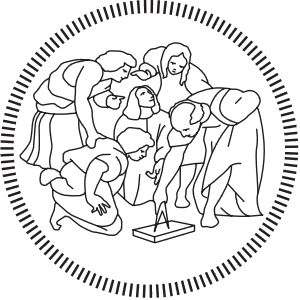
\includegraphics[scale=0.1]{etc/logo.png}
%	\end{textblock*}
%}

\begin{frame} %#02
	\frametitle{Ordinary differential equations (ODE)}
	\begin{itemize}
		\item Spacial coordinates: $\yy \in \RR^n$
		\item Time: $t \in I = [t_0, t_F] \subset \RR$
		\item Equation function: $f(t,\yy): I \times \RR^n \to \RR^n, \quad f \in C^1$
		\item Initial value: $t_0 \in I, \quad \yy_0 \in \RR^n$
	\end{itemize}
	\vspace{15pt}
	\pause
	\begin{center}
		\textbf{Initial Value Problem (IVP)}: \\[15pt]
		find a $C^1$ function $\yy(t): I \to \RR^n$ that solves
		$$
		\begin{cases}
		\yy'(t) = f( t,\yy(t) ) \qquad \text{with } t \in I \\
		\yy(t_0) = \yy_0
		\end{cases}
		$$
		(first order ODE)
		%Ordinary: derive only wrt y
		%Higher-order EDOs can be reduced to a set of order 1 EDOs
	\end{center}
\end{frame}

\begin{frame} %#03
	\frametitle{Existence and uniqueness of solution}
	\begin{itemize}
		\item Guaranteed under \textit{Lipschitz continuity}:
			$$ \abs{f(t,\yy_1) - f(t,\yy_2)} \le \, L \abs{\yy_1 - \yy_2}
			\qquad \forall t \in U(t_0), \ \ \yy_1, \yy_2 \in U(\yy_0) $$
		\item Can be extended to the whole $I \times \RR^n$
		\pause
		\item But computing $\yy$ analitically may be difficult, impossible, or inefficient \\[30pt]
			\begin{center}
			$\implies$ \textbf{numerical approximations}
		\end{center}
	\end{itemize}
	% Applications of ODEs: everywhere
\end{frame}

\begin{frame} %#04
	\frametitle{General features of iterative methods}
	\begin{itemize}
		\item Discretization of time into $N$ intervals: $t_0, \ t_1, \ \dots, \ t_{N} = t_F$
		\item $n = 0, 1, \dots, N$
		\item Discretization step: $t_{n+1} = t_n + h$
		\pause
		\item Vectorial approximation of $\yy$:
		\begin{center}
			$\uu_0 = \yy_0, \uu_1, \dots, \uu_{N} \in \RR^n$
		\end{center}
		\item $\uu_n$ is iteratively updated $\forall n = 1, \dots, N-1$
	\end{itemize}
\end{frame}

\begin{frame}
	\frametitle{Single-step methods} %#05
	\begin{itemize}
		\item $\uu_{n+1}$ depends directly only on the one previous step $\uu_{n}$
		\item General updating scheme (with generic increment function $\phi$):
		$$ \uu_{n+1} = \uu_{n} + h \ \phi(t_n, \, h, \, \uu_n, \, \uu_{n+1}, \, f) $$
		\pause
		\item \textit{Explicit} methods: $\uu_{n+1}$ does not appear in $\phi$
		\item \textit{Implicit} methods: $\uu_{n+1}$ appears in $\phi$
		\begin{center}
			\vspace{-5pt}
			$\implies$ nonlinear equations
		\end{center}
	\end{itemize}
\end{frame}


\begin{frame} %#06
	\frametitle{Runge-Kutta methods}
	\begin{itemize}
		\item Family of single-step methods
		\item Weighted average of $s$ evaluations (\textit{stages}) of $f$:
		$$ \uu_{n+1} = \uu_{n} + h \sum_{i=1}^s b_i \kk_i \quad \text{with} $$
		\vspace{-6pt}
		$$ \kk_i = f(t_0 + c_i h, \ \uu_n + \sum_{j=1}^s a_{ij} \kk_j) $$
		\pause
		\item \textit{Butcher tableau}:
		\begin{center}
			\begin{tabular}{c|ccc}
				$c_1$ & $a_{11}$ & $\dots$ & $a_{1s}$ \\
				\vdots & & $\ddots$ & \\
				$c_s$ & $a_{s1}$ & & $a_{ss}$ \\
				\hline
				& $b_1$ & $\dots$ & $b_s$
			\end{tabular}
		with $c_i = \sum_j a_{ij}$
		\pause
		\end{center}
		\item $O(s n^2)$ if $f$ linear
		\item Explicit if $[a_{ij}]_{ij}$ is lower triangular
	\end{itemize}
\end{frame}


\begin{frame} %#07
	\frametitle{Examples of explicit RK variants}
	\begin{itemize}
		\item \textbf{Forward Euler} (FE):
		$$ a = 0, b = 1, c = 0 $$
		$$ \uu_{n+1} = \uu_{n} + h f(t_n, \uu_n) $$
		\item RK4 (standard):
		\begin{tabular}{c|cccc}
			$0$ & & & & \\
			$\frac 1 2$ & $\frac 1 2$ & & & \\
			$\frac 1 2$ & & $\frac 1 2$ & & \\
			$1$ & & & 1 & \\
			\hline
			& $\frac 1 6$ & $\frac 1 3$ & $\frac 1 3$ & $\frac 1 6$
			\end{tabular}
		\item Heun:
		\begin{tabular}{c|cc}
			$0$ &     & \\
			$1$ & $1$ & \\
			\hline
			    & $\frac 1 2$ & $\frac 1 2$
			\end{tabular}	
	\end{itemize}
\end{frame}


\begin{frame} %#08
	\frametitle{Examples of implicit RK variants}
	\begin{itemize}
		\item Iserles-Nørsett:
		\begin{tabular}{c|cccc}
			$\frac{3-\sqrt{3}}{6}$ & $\frac{5}{12}$ & $\frac{1-2\sqrt{3}}{12}$ & & \\
			$\frac{3+\sqrt{3}}{6}$ & $\frac{1+2\sqrt{3}}{12}$ & $\frac{5}{12}$ & & \\
			$\frac{3-\sqrt{3}}{6}$ & & & $\frac{1}{2}$ & $-\frac{\sqrt{3}}{6}$ \\
			$\frac{3+\sqrt{3}}{6}$ & & & $\frac{\sqrt{3}}{6}$ & $\frac{1}{2}$ \\
			\hline
			& $\frac{3}{2}$ & $\frac{3}{2}$ & $1$ & $1$
			\end{tabular}
		%TODO: do we need another one?	
	\end{itemize}
\end{frame}


\begin{frame} %#09
	\frametitle{Convergence analysis}
	\begin{itemize}
		\item Convergence $\to$ absolute error: $\norm{y_n - u_n} \simeq O(h^q)$
		\item Consistence $\to$ truncation error: $\max_n \norm{\tau_n(h)} \simeq O(h^q)$
		\item Stability $\to$ absolute error of perturbed numerical solution $z_n$:
		$$ 	norm{z_n-u_n} < C \varepsilon \qquad
		\text{given perturbation } < \varepsilon, \text{for some } h_0 $$
	\end{itemize}
	\pause
	Examples:
	\begin{itemize}
		\item Forward and backward Euler are order 1 methods
		\item Under reasonable Lipschitz continuity assumptions on $\phi$, and if the method is also single-step and consistent, then it's convergent
	\end{itemize}
\end{frame}


\begin{frame} %#10
\frametitle{Convergence of RK}
	\begin{itemize}
		\item Runge-Kutta is consistent iff $\sum_i b_i = 1$ $\implies$
		\item Therefore, it's convergent via the previous result
		\item Steep limitations on order of convergence:
		\begin{itemize}
			\item Maximum order is the number of stages
			\item If $s \ge 5$, equality cannot be achieved in explicit variants
		\end{itemize}
	\end{itemize}
	\begin{tabular}{c|cccc}
		order & 5 & 6 & 7 & 8\\
		\hline
		minimum $s$ & 6 & 7 & 9 & 11 
	\end{tabular}
\end{frame}



\begin{frame} %#11
\frametitle{Model problem analysis (in $\RR$)}
	$$ y'(t) = \lambda(t) y \qquad \text{with } t > 0, \ y(0) = y_0 $$
	\begin{itemize}
		\item Absolute stability: $u_n \to 0$ as $n \to +\infty$
		\item FE is absolutely stable iff $h < \frac{2}{\max_t \abs{\lambda(t)}} $
		\item Be is absolutely stable $\forall h$
	\end{itemize}
	% Problem: number of intervals N -> +inf even with h fixed, i.e. not
	% tending to 0
\end{frame}


\begin{frame} %#12
\frametitle{Absolute stability controls oscillations}
\begin{itemize}
	\item Generalized model problem:
	$$ y'(t) = \lambda(t) y(t) + r(t) \quad \text{with } t > 0, y(0) = \boldsymbol 1,
	\lambda(t)<0 \in C^0 \cap L^\infty,  r(t) \in C^0 $$
	\item No absolute stability, but...
	\item Absolutely stable Forward Euler case:
	\begin{itemize}
		\item $\abs{z_n - u_n} = \dots$ %TODO
		\item $\abs{z_n - u_n} < \sup_k(\abs{\rho_k}) \cdot A(\lambda_k), \ \forall n,h$ %TODO check
		\item This can also be generalized to any IVP
	\end{itemize}
\end{itemize}
%  TODO: reasons to use adaptive step?
\end{frame}


\begin{frame} %#13
	\frametitle{Adaptive methods}
	Step is updated at every iteration, based on the trend of the solution
	\begin{itemize}
		\item Small $h$ near steep slopes, large $h$ near flat points %TODO check
		% In model problem, lam(t) decreasing => function is flat %TODO check
		\item \textit{A posteriori} estimate of error is needed
		\item Compute both two-round solution with $\frac{h}{2}$ and single-round solution with $h$
	\end{itemize}
\end{frame}

\begin{frame} %#14
	\frametitle{Consistency of adaptive methods}
	\begin{itemize}
		\item Forward Euler: truncation errors are
		$$ e_h = h^2/2 y"(\xi), \qquad e_{h/2} = h^2/8 y"(\eta) \cdot 2 + o(h^2) $$
		$$\implies \abs{u_{h/2} - u_h} \simeq \abs{e_(h/2)} \simeq h^2/4 \abs{y"(\widehat\eta)}
		+ o(h^2) \stackrel{\downarrow}{<} \frac{\varepsilon}{2}
		\quad \text{(tolerance)} $$
		\item Runge-Kutta %TODO!!!!!!!!!
	\end{itemize}
\end{frame}


\begin{frame} %#15
	Code structure %TODO put big ass title
\end{frame}


\begin{frame} %#16
	\frametitle{Code structure}
	
\includegraphics[scale=0.3]{etc/test.jpg}
\end{frame}


\begin{frame} %#17
	\frametitle{Programming choices}
	\begin{itemize}
		\item Separate FE class is more efficient than RK specialized class
		% Moreover, the adaptive RK error is computed differently because there
		% are some unknown (in the general case) quantities that need to be
		% estimated
		
\includegraphics[scale=0.3]{etc/test.jpg}
		\item Adaptive \verb|single_step()| class methods are not efficient
	\end{itemize}
	
\end{frame}

\begin{frame} %#18
	\frametitle{Results}
	
\includegraphics[scale=0.3]{etc/test.jpg}
\end{frame}

\begin{frame} %#19
	\frametitle{Bibliography}
	\begin{thebibliography}
		\setbeamertemplate{bibliography item}[book] % or [online] or [article]
		\bibitem ItemB Quarteroni, Sacco, Saleri, Gervasio, \textit{Matematica numerica}
		\bibitem Quarteroni, Saleri, \textit{Calcolo scientifico}
		\bibitem Solodushkin, Iumanova, \textit{Parallel Numerical Methods for Ordinary Differential Equations: a Survey}
		\bibitem Podhaisky, \textit{Parallel two-step Runge-Kutta methods}	
	\end{thebibliography}
\end{frame}

\end{document}




\begin{frame}
	\frametitle{Title}
	
	\begin{itemize}
		\item 
	\end{itemize}
\end{frame}
